
\documentclass[11pt, spanish]{article}
\usepackage[T1]{fontenc}
\usepackage[utf8]{inputenc}
\usepackage{amsmath}
\usepackage{amssymb}
% \usepackage{hyperref}
\usepackage{graphicx}
\usepackage{tikz}
\usetikzlibrary{shapes,arrows,positioning,calc}
\usepackage{geometry}
\geometry{
	left=15mm,
	right=15mm,
	top=20mm,
	bottom=20mm,
}

\title{Controles - Taller Clase 7}
\author{Pontificia Universidad Javeriana, Bogotá\\Profesor: Ing. Gerardo Becerra, Ph.D.}
\date{Marzo 18 de 2020}

\begin{document}
	\maketitle

\begin{enumerate}

 	\item El sistema de control mostrado en la figura representa el control de velocidad de un motor DC, usando un tacómetro de precisión. Se desea mantener una alta precisión en estado estacionario para el control de velocidad. Diseñe un compensador de adelanto para que se satisfagan los siguientes requerimientos: $PO = 10\%$, $T_s \leq 1.5$ s.
	 \begin{figure}[h]
	 	\centering
	 	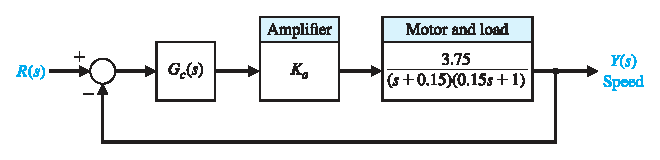
\includegraphics[width=13cm]{taller_ejericio1.eps}
	 \end{figure}

	\item Un sistema de control con retroalimentación unitaria tiene la siguiente función de transferencia de lazo abierto:
		\begin{equation*}
			G_c(s)G(s) = G_c(s)\frac{5}{s(s^2+5s+12)}
		\end{equation*}
		\begin{itemize}
			\item Diseñe un compensador de atraso usando el LGR tal que la constante de velocidad sea incrementada en 10.
			\item Compare la respuesta paso del sistema no compensado con la del sistema compensado.
		\end{itemize}

	\item Un sistema de control con retroalimentación unitaria tiene la siguiente función de transferencia de lazo abierto:
		\begin{equation*}
			G_c(s)G(s) = G_c(s)\frac{160}{s^2}
		\end{equation*}
		\begin{itemize}
			\item Diseñe un compensador de adelanto-atraso usando el LGR tal que los siguientes requerimientos sean satisfechos: $PO \leq 5\%$, $T_s \leq 1$ s, $K_a >= 7500$ (constante de aceleración).
			\item Compare la respuesta paso del sistema no compensado con la del sistema compensado.
		\end{itemize}
 
\end{enumerate}

\end{document}